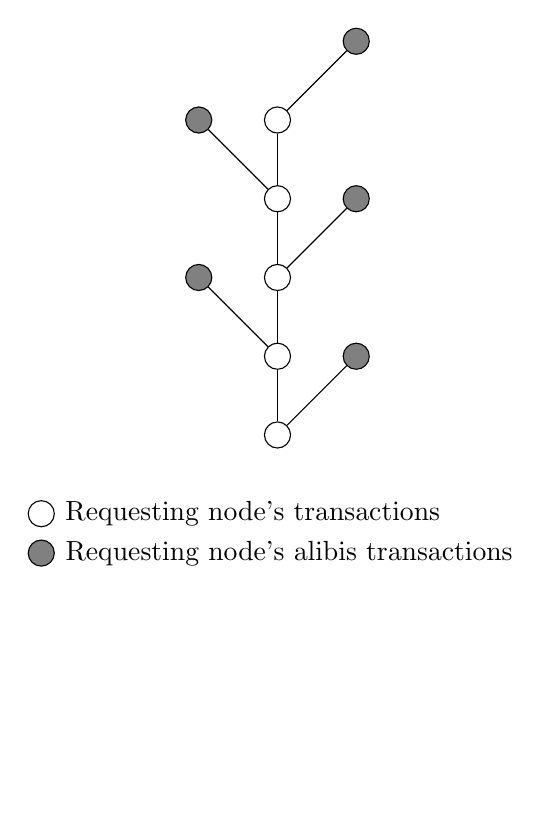
\begin{tikzpicture}[every node/.style={draw,shape=circle,fill=black}]

\node[fill=white] (A) at (0,0) {};
\node[fill=white] (B) at (0,1) {};
\node[fill=white] (C) at (0,2) {};
\node[fill=white] (D) at (0,3) {};
\node[fill=white] (E) at (0,4) {};

\node[fill=white,label=right:Requesting node's transactions] (L1) at (-3,-1) {};
\node[fill=gray,label=right:Requesting node's alibis transactions] (L2) at (-3,-1.5) {};

\draw (A) -- (B) (B) -- (C) (C) -- (D) (D) -- (E);

\node[fill=gray] (F) at (1,1) {};
\draw (A) -- (F);

\node[fill=gray] (G) at (-1,2) {};
\draw (B) -- (G);

\node[fill=gray] (H) at (1,3) {};
\draw (C) -- (H);

\node[fill=gray] (I) at (-1,4) {};
\draw (D) -- (I);

\node[fill=gray] (J) at (1,5) {};
\draw (E) -- (J);

\end{tikzpicture}